\section{Experimental results}\label{sec:results}

To give comparative results on the quality of the initialisation processes 
defined in
Sections~\ref{sec:init},~\ref{sec:proposed-method}~\&~\ref{sec:preferences},
four well-known, categorical, labelled datasets \--- soybean, mushroom, breast
cancer, and zoo animal \--- will be clustered by the \(k\)-modes algorithm with
each of the initialisation processes using their respective number of classes as
the number of clusters. These datasets have been chosen to fall in line with the
established literature, and for their relative sizes and complexities.

Typically, the quality of a clustering algorithm is measured by its performance
at classifying datasets~\cite{Cao2009, Huang1998, Olaode2014}. In this work,
however, we will not follow this approach since our motivation is to compare the
quality of the clustering produced when using these initialisation methods. So,
for the purposes of measuring the performance of our various initialisation
methods as parts of a clustering algorithm, we will make use of internal metrics
that are independent of any external information such as a class labelling.
This family of metrics are built up from two characteristics of the clusters
found: cohesion and separation. Cluster cohesion is effectively the summed,
within-cluster variation or dissimilarity of its points, whereas a cluster's
separation is a sum of the distances between all points in the cluster and every
other point not in the cluster. In this analysis, we will make use of two
internal measures for cluster validity: our cost function from
Definition~\ref{def:cost} and the average silhouette coefficient, or silhouette
score, of our clustering, defined below. 

\begin{definition}\label{def:silhouette}
    Let \textbf{X} be a dataset and consider a clustering of \textbf{X} into
    \(k\) parts, denoted by \(C = \left\{C_1, \ldots, C_k\right\}\). For each
    \(X^{(i)} \in \textbf{X}\), we define the following two quantities:
    \begin{itemize}
        \item Let \(a\left(X^{(i)}\right)\) denote the average dissimilarity
            between \(X^{(i)}\) and every other point in its cluster. Without
            loss of generality, let \(X^{(i)} \in C_l\). Then:
            \[
                a\left(X^{(i)}\right) := \frac{1}{|C_l|} D\left(C_l,
                X^{(i)}\right)
            \]
        \item Let \(b\left(X^{(i)}\right)\) denote the lowest average 
            dissimilarity between \(X^{(i)}\) and all other points in each
            cluster other than \(C_l\). That is:
            \[
                b\left(X^{(i)}\right) := \min_{l' \neq l} \left\{
                \frac{1}{|C_{l'}|} D\left(C_{l'}, X^{(i)}\right) \right\}
            \]
    \end{itemize}

    With these quantities we define, for each point in our datset, their
    \emph{silhouette coefficient}, denoted by \(s(X^{(i)})\):
    \[
        s(X^{(i)}) := \frac{b\left(X^{(i)}\right) -
        a\left(X^{(i)}\right)}{\max\left\{a\left(X^{(i)}\right),
        b\left(X^{(i)}\right)\right\}}
    \]

    The \emph{silhouette score} of a clustering \(C\) is simply the average of
all the silhouette coefficients. Silhouette scores take value in the range
\([-1, 1]\). Negative scores generally suggest that elements in the data have
been mis-clustered since there exists a closer cluster centre than its own.
Values around 0 indicate overlapping clusters, whereas silhouette scores close
to 1 suggest well-separated and effective clusters.
\end{definition}


\subsection{The datasets}\label{subsec:datasets}

As stated above, the datasets being used for this work are well-known and openly
available. Below is a summary of their properties and access links for each.

\subsubsection*{Soybean}

The soybean dataset describes 35 characteristics of 307 soybean instances to
classify which disease is present. The attributes are encoded numerically as
integers but will be considered as strings for this analysis.
The diseases form .8 classes, though the first 15 are the only ones used since
they contain a considerable number of instances each~\cite{Soybean}. 
Available~at:~\url{https://archive.ics.uci.edu/ml/datasets/Soybean+(Large)}.

\subsubsection*{Mushroom}

The mushroom dataset was constructed to classify 8124 mushroom instances forming
23 species found in North America into two classes: edible and poisonous. The
attributes describe the physical characteristics and habitat of the mushrooms,
and are encoded as strings~\cite{Mushroom}. Available~at:~\url{https://archive.
ics.uci.edu/ml/datasets/mushroom}.

\subsubsection*{Breast cancer}

Wisconsin University constructed the breast cancer dataset using a decision tree
with linear programming as a diagnostic tool. The features were created using
digital images of a fine needle aspirate of a breast mass to describe the
structure of cell nuclei. There are 699 instances and 32 attributes in total.
Available~upon~request~to~members~of~the~academic~community~at:~\url{https://
archive.ics.uci.edu/ml/datasets/Breast+Cancer+Wisconsin+(Diagnostic)}.

\subsubsection*{Zoo animal}

The zoo animal dataset is an entirely artificial dataset used to classify 101
animals into 7 classes, those being mammal, reptile, amphibian, bird, fish,
insect, and crustacean. The 17 attributes include the name of the animal and a
series of Boolean variables describing characteristics and the habitat of the
animals. Available~at:~\url{http://archive.ics.uci.edu/ml/datasets/zoo}.

\subsection{Results}\label{subsec:results}

In this section, two sets of results will be considered. The first are the more
classically seen tables of metrics defined above, and the latter are a
collection of plots showing the descent in the cost function of the \(k\)-modes
algorithm over time. In either case, results are generated using the Python
library \href{https://github.com/nicodv/kmodes}{\texttt{kmodes}} to which the
proposed method has been added as another initialisation method. The number of
clusters to be determined, \(k\), is chosen as the number of classes associated
with each dataset. Note that this value may not be optimal (as suggested by the
relatively low silhouette scores in most cases), and that the class variable is
not considered in the running of the algorithm.

\subsubsection{Metric results}

Each of the tables of results given below were obtained by running the
\(k\)-modes algorithm 25 times with each initialisation method on the dataset in
question. For each of these 25 runs, the simulation is seeded to make the
results reproducible.

At each run of the experiment the number of epochs to termination, the initial
and final costs, and the average silhouette score were recorded for the
clustering found. These metrics are summarised below in
Tables~\ref{tab:soybean_results}~\--~\ref{tab:zoo_animal_results} by their mean
and median values, and their standard deviation over the 25 runs.

\singlespacing%
\begin{table}[H]
    \centering
    \resizebox{.9\textwidth}{!}{%
        \begin{tabular}{llrrrr}
\toprule
Initialisation & {} &  No. of iterations &  Initial cost &  Final cost &  Silhouette score \\
\midrule
Cao & mean &             2.0000 &     1574.0000 &   1314.0000 &            0.2349 \\
    & median &             2.0000 &     1574.0000 &   1314.0000 &            0.2349 \\
    & std &             0.0000 &        0.0000 &      0.0000 &            0.0000\\
\midrule
Huang & mean &             3.7600 &     1795.4400 &   1455.3200 &            0.1212 \\
    & median &             4.0000 &     1830.0000 &   1428.0000 &            0.1234 \\
    & std &             1.0520 &      131.9621 &     72.7637 &            0.0357 \\
\midrule
Matching Best & mean &             3.6800 &     1773.2400 &   1449.6400 &            0.1205 \\
    & median &             3.0000 &     1781.0000 &   1443.0000 &            0.1193 \\
    & std &             1.1075 &      118.8992 &     63.0971 &            0.0247 \\
\midrule
Matching Random & mean &             3.8800 &     1774.3600 &   1438.8000 &            0.1237 \\
    & median &             4.0000 &     1780.0000 &   1431.0000 &            0.1291 \\
    & std &             1.0924 &      121.9911 &     54.0301 &            0.0234 \\
\midrule
Matching Worst & mean &             4.0400 &     1774.9600 &   1431.8400 &            0.1290 \\
    & median &             4.0000 &     1777.0000 &   1430.0000 &            0.1291 \\
    & std &             1.0985 &      123.0411 &     53.9859 &            0.0248 \\
\midrule
Random & mean &             3.6800 &     1638.8000 &   1351.2400 &            0.1608 \\
    & median &             3.0000 &     1626.0000 &   1345.0000 &            0.1620 \\
    & std &             1.1804 &       98.2480 &     36.3126 &            0.0312 \\
\bottomrule
\end{tabular}

    }
    \captionof{table}{Summative metric results for the soybean dataset with
    \(k=15\).}\label{tab:soybean_results}\vspace{20pt}

    \resizebox{.9\textwidth}{!}{%
        \begin{tabular}{llrrrr}
\toprule
Initialisation & {} &  No. of iterations &  Initial cost &  Final cost &  Silhouette score \\
\midrule
Cao & mean &             2.0000 &    63242.0000 &  62644.0000 &            0.2517 \\
    & median &             2.0000 &    63242.0000 &  62644.0000 &            0.2517 \\
    & std &             0.0000 &        0.0000 &      0.0000 &            0.0000 \\
\midrule
Huang & mean &             2.8400 &    75107.8400 &  63231.8400 &            0.2274 \\
    & median &             3.0000 &    76026.0000 &  63002.0000 &            0.2179 \\
    & std &             0.9866 &     5864.1758 &   1059.4049 &            0.0332 \\
\midrule
Matching Best & mean &             2.8400 &    74822.2800 &  63319.5600 &            0.2209 \\
    & median &             3.0000 &    75192.0000 &  63015.0000 &            0.2179 \\
    & std &             1.0279 &     4914.2731 &   1186.2087 &            0.0345 \\
\midrule
Matching Random & mean &             2.8400 &    74822.2800 &  63319.5600 &            0.2209 \\
    & median &             3.0000 &    75192.0000 &  63015.0000 &            0.2179 \\
    & std &             1.0279 &     4914.2731 &   1186.2087 &            0.0345 \\
\midrule
Matching Worst & mean &             2.8400 &    74822.2800 &  63319.5600 &            0.2209 \\
    & median &             3.0000 &    75192.0000 &  63015.0000 &            0.2179 \\
    & std &             1.0279 &     4914.2731 &   1186.2087 &            0.0345 \\
\midrule
Random & mean &             2.6400 &    78345.8400 &  63824.8000 &            0.2243 \\
    & median &             2.0000 &    78603.0000 &  63155.0000 &            0.2281 \\
    & std &             0.8103 &     6146.4742 &   1684.9847 &            0.0391 \\
\bottomrule
\end{tabular}

    }
    \captionof{table}{Summative metric results for the mushroom dataset with
    \(k=2\).}\label{tab:mushroom_results}
\end{table}

\begin{table}[H]
    \centering
    \resizebox{.9\textwidth}{!}{%
        \begin{tabular}{llrrrr}
\toprule
Initialisation & {} &  No. of iterations &  Initial cost &  Final cost &  Silhouette score \\
\midrule
Cao & mean &             3.0000 &     3546.0000 &   3250.0000 &            0.3453 \\
    & median &             3.0000 &     3546.0000 &   3250.0000 &            0.3453 \\
    & std &             0.0000 &        0.0000 &      0.0000 &            0.0000 \\
\midrule
Huang & mean &             2.0400 &     3809.3200 &   3428.3200 &            0.1655 \\
    & median &             2.0000 &     3846.0000 &   3492.0000 &            0.0933 \\
    & std &             0.4546 &      206.2981 &    151.9832 &            0.1595 \\
\midrule
Matching Best & mean &             2.0400 &     3804.7200 &   3386.4000 &            0.1943 \\
    & median &             2.0000 &     3803.0000 &   3257.0000 &            0.3439 \\
    & std &             0.4546 &      177.0794 &    146.2635 &            0.1681 \\
\midrule
Matching Random & mean &             2.0400 &     3804.7200 &   3386.4400 &            0.1940 \\
    & median &             2.0000 &     3803.0000 &   3257.0000 &            0.3439 \\
    & std &             0.4546 &      177.0794 &    146.2247 &            0.1677 \\
\midrule
Matching Worst & mean &             2.0400 &     3804.7200 &   3386.4400 &            0.1940 \\
    & median &             2.0000 &     3803.0000 &   3257.0000 &            0.3439 \\
    & std &             0.4546 &      177.0794 &    146.2247 &            0.1677 \\
\midrule
Random & mean &             2.0400 &     4150.8000 &   3349.9200 &            0.2338 \\
    & median &             2.0000 &     3682.0000 &   3250.0000 &            0.3453 \\
    & std &             0.3512 &      828.8702 &    136.8819 &            0.1631 \\
\bottomrule
\end{tabular}

    }
    \captionof{table}{Summative metric results for the breast cancer dataset
    with \(k=2\).}\label{tab:breast_cancer_results}\vspace{20pt}

    \resizebox{.9\textwidth}{!}{%
        \begin{tabular}{llrrrr}
\toprule
    &      &  No. of iterations &  Initial cost &  Final cost &  Silhouette score \\
Initialisation & {} &                    &               &             &                   \\
\midrule
Cao & mean &             2.0000 &     1574.0000 &   1314.0000 &            0.2349 \\
    & median &             2.0000 &     1574.0000 &   1314.0000 &            0.2349 \\
    & std &             0.0000 &        0.0000 &      0.0000 &            0.0000 \\
Huang & mean &             3.7600 &     1795.4400 &   1455.3200 &            0.1212 \\
    & median &             4.0000 &     1830.0000 &   1428.0000 &            0.1234 \\
    & std &             1.0520 &      131.9621 &     72.7637 &            0.0357 \\
Matching Best & mean &             3.6800 &     1773.2400 &   1449.6400 &            0.1205 \\
    & median &             3.0000 &     1781.0000 &   1443.0000 &            0.1193 \\
    & std &             1.1075 &      118.8992 &     63.0971 &            0.0247 \\
Matching Random & mean &             3.8800 &     1774.3600 &   1438.8000 &            0.1237 \\
    & median &             4.0000 &     1780.0000 &   1431.0000 &            0.1291 \\
    & std &             1.0924 &      121.9911 &     54.0301 &            0.0234 \\
Matching Worst & mean &             4.0400 &     1774.9600 &   1431.8400 &            0.1290 \\
    & median &             4.0000 &     1777.0000 &   1430.0000 &            0.1291 \\
    & std &             1.0985 &      123.0411 &     53.9859 &            0.0248 \\
Random & mean &             3.6800 &     1638.8000 &   1351.2400 &            0.1608 \\
    & median &             3.0000 &     1626.0000 &   1345.0000 &            0.1620 \\
    & std &             1.1804 &       98.2480 &     36.3126 &            0.0312 \\
\bottomrule
\end{tabular}

    }
    \captionof{table}{Summative metric results for the zoo animal dataset with
    \(k=7\).}\label{tab:zoo_animal_results}
\end{table}
\doublespacing%

\subsubsection{Epoch costs}

The epoch-cost plots in this section were created by setting an initial seed for
each initialisation method and then running the \(k\)-modes algorithm 25 times.
Of these runs, the best set of costs is then chosen by their final cost and
plotted.

Note that in each figure, dotted lines indicate the established initialisation
methods whilst solid lines are used for the proposed method.

\begin{figure}[h!]
    \centering
    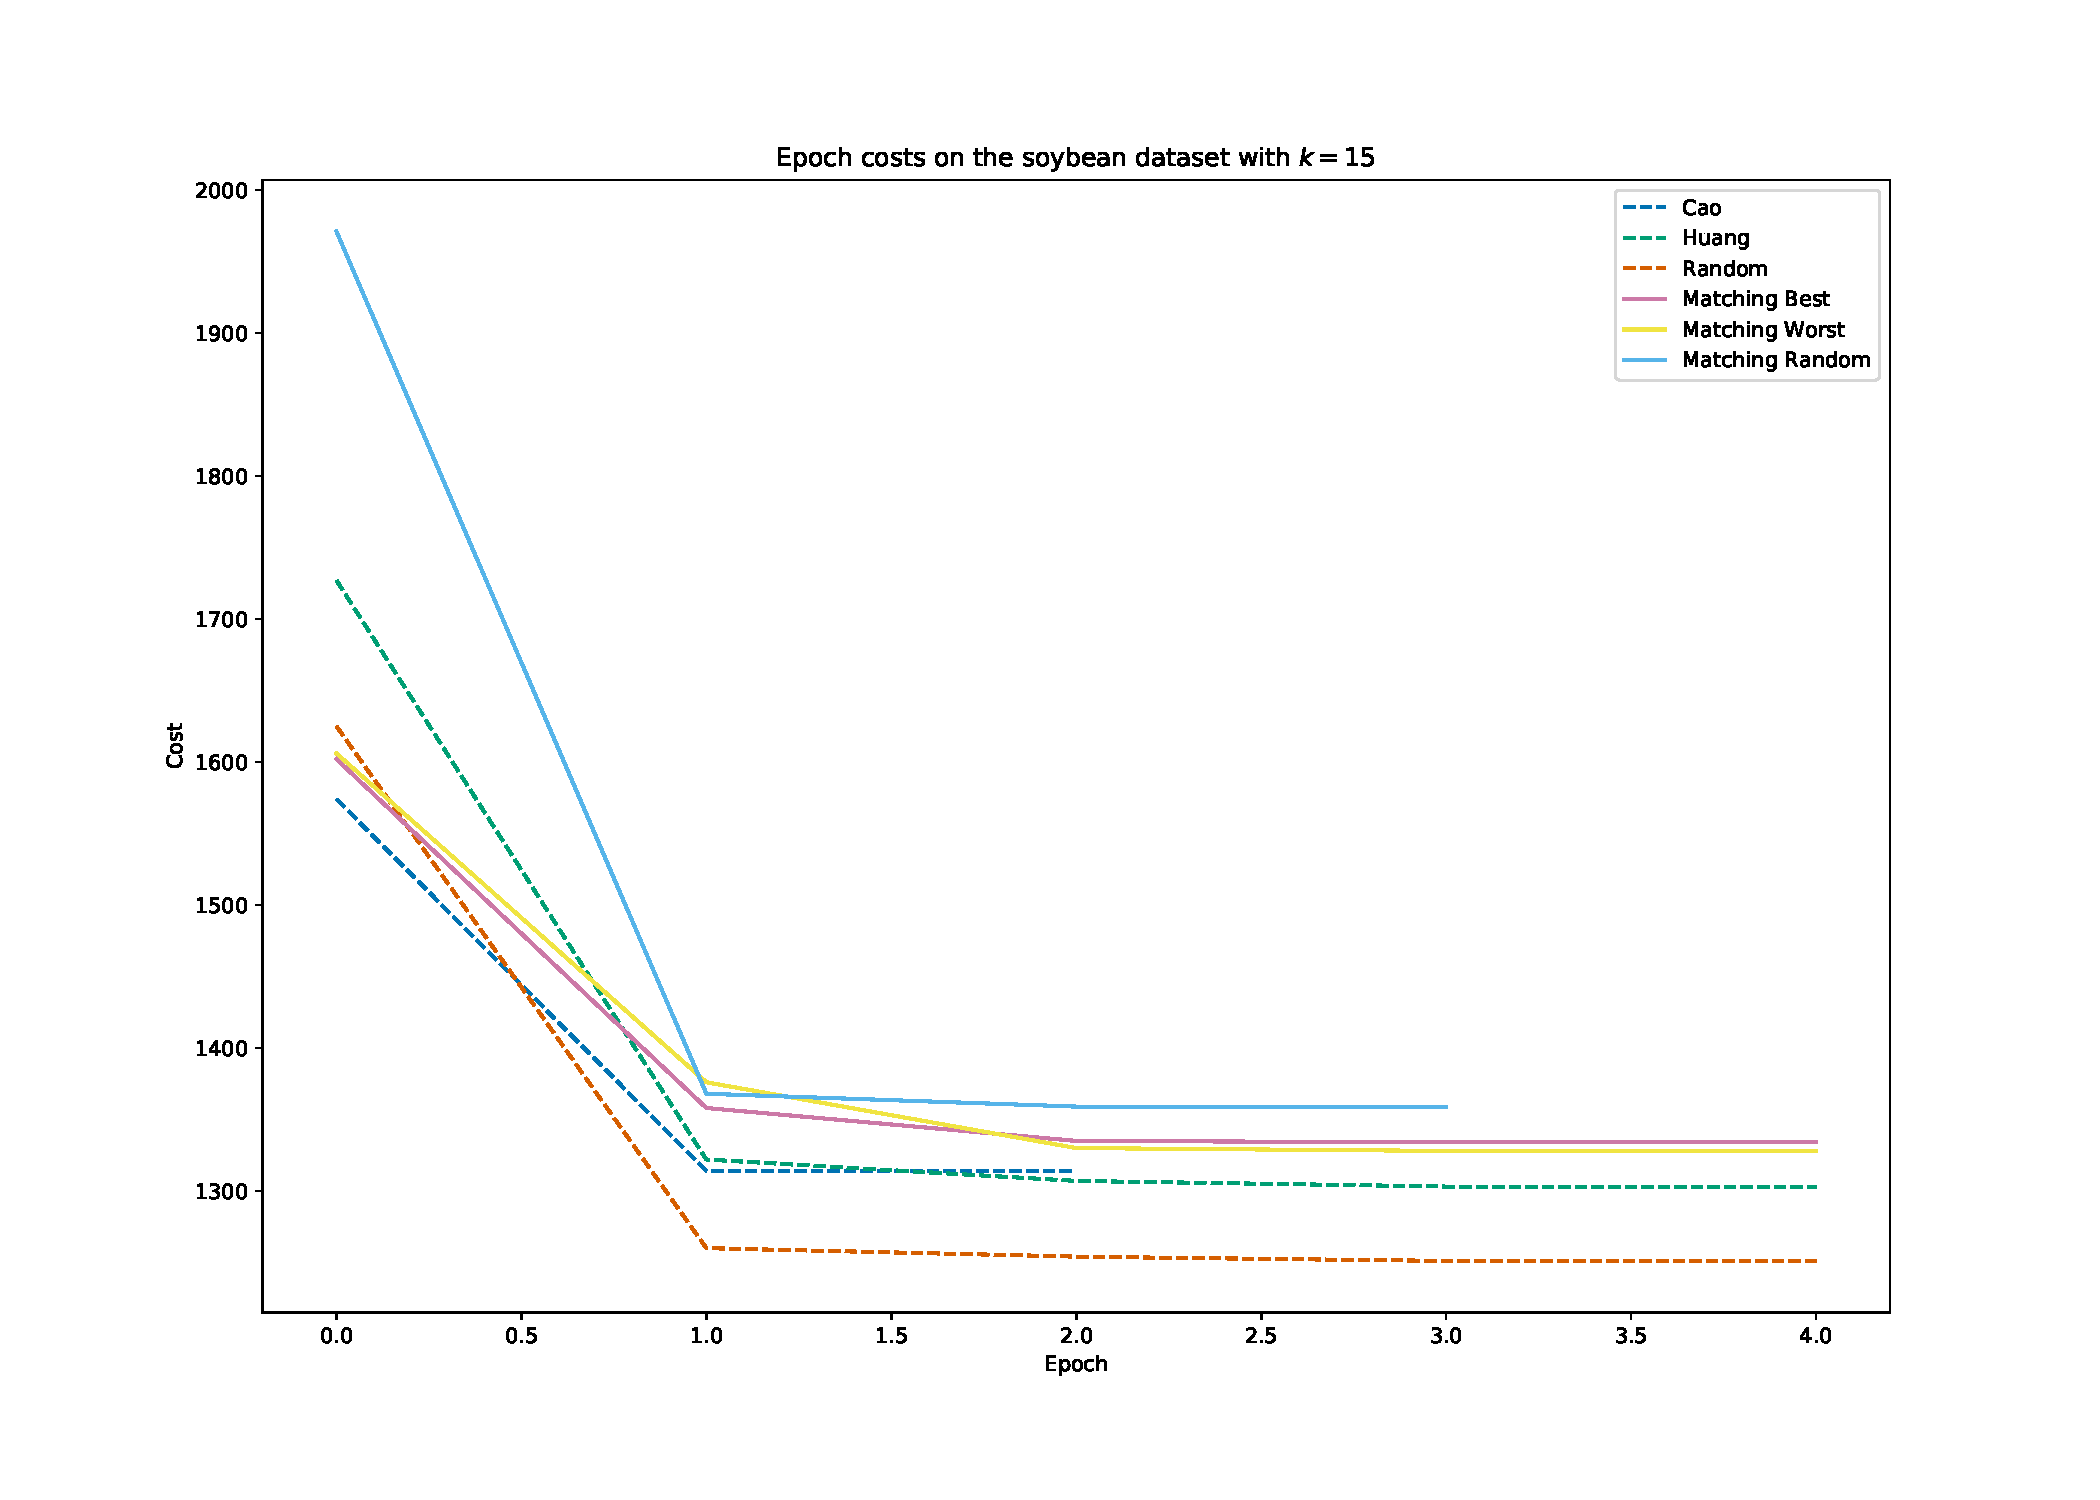
\includegraphics[width=.8\textwidth]{./img/epoch_plot_soybean.pdf}
\end{figure}

\begin{figure}[h!]
    \centering
    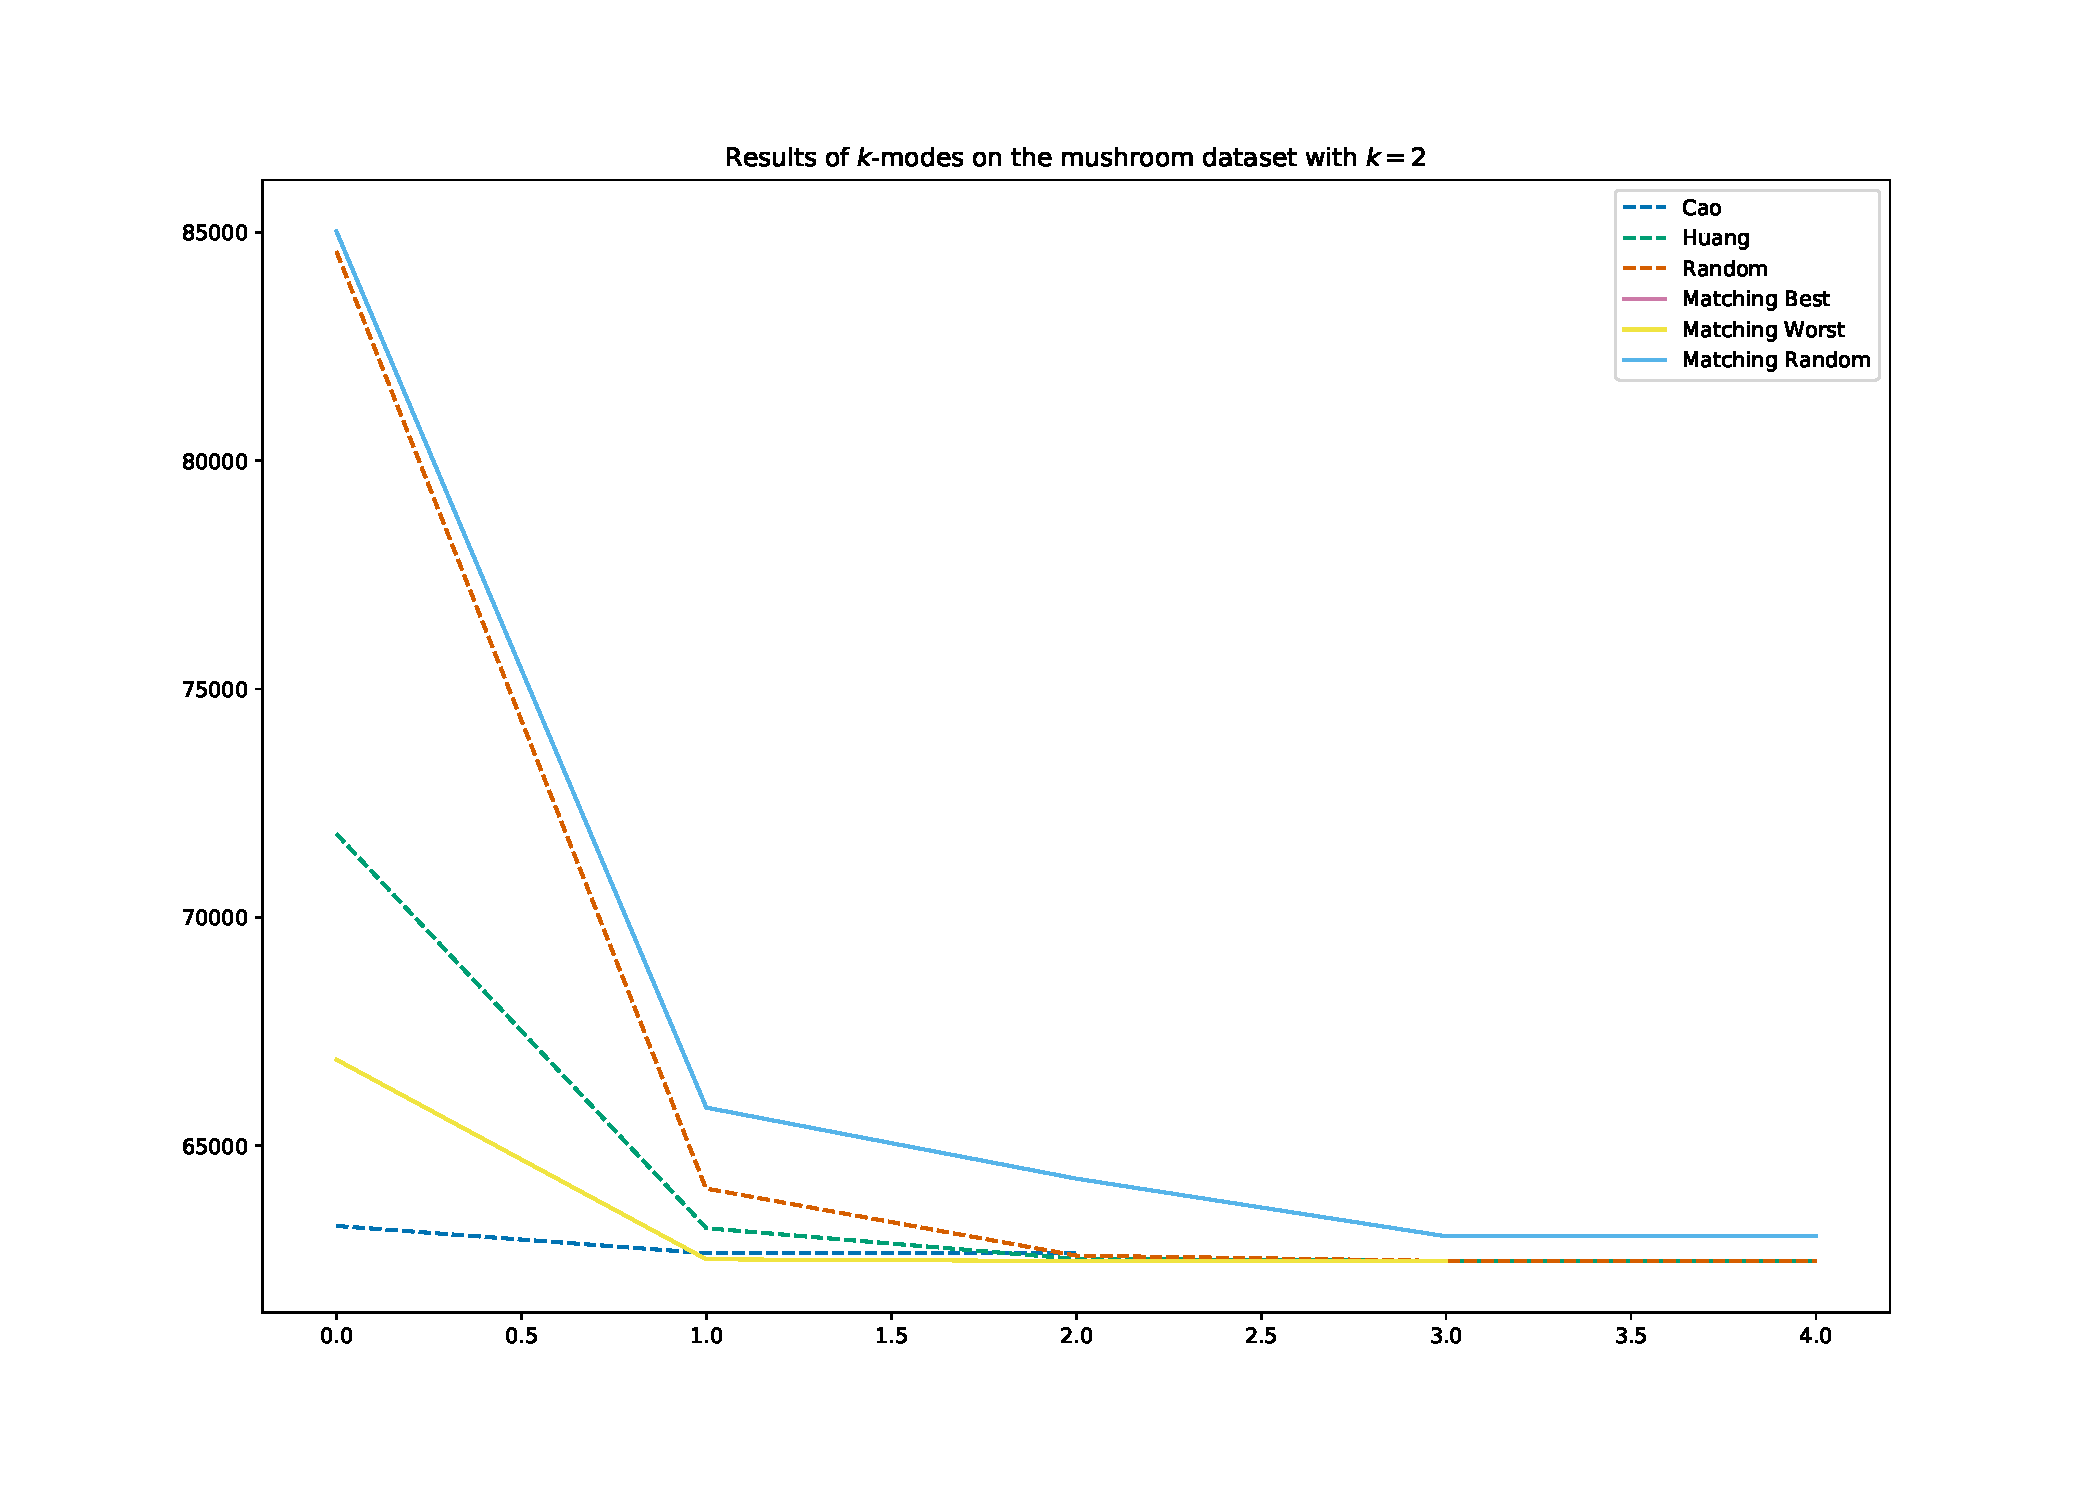
\includegraphics[width=.8\textwidth]{./img/epoch_plot_mushroom.pdf}
\end{figure}

\begin{figure}[h!]
    \centering
    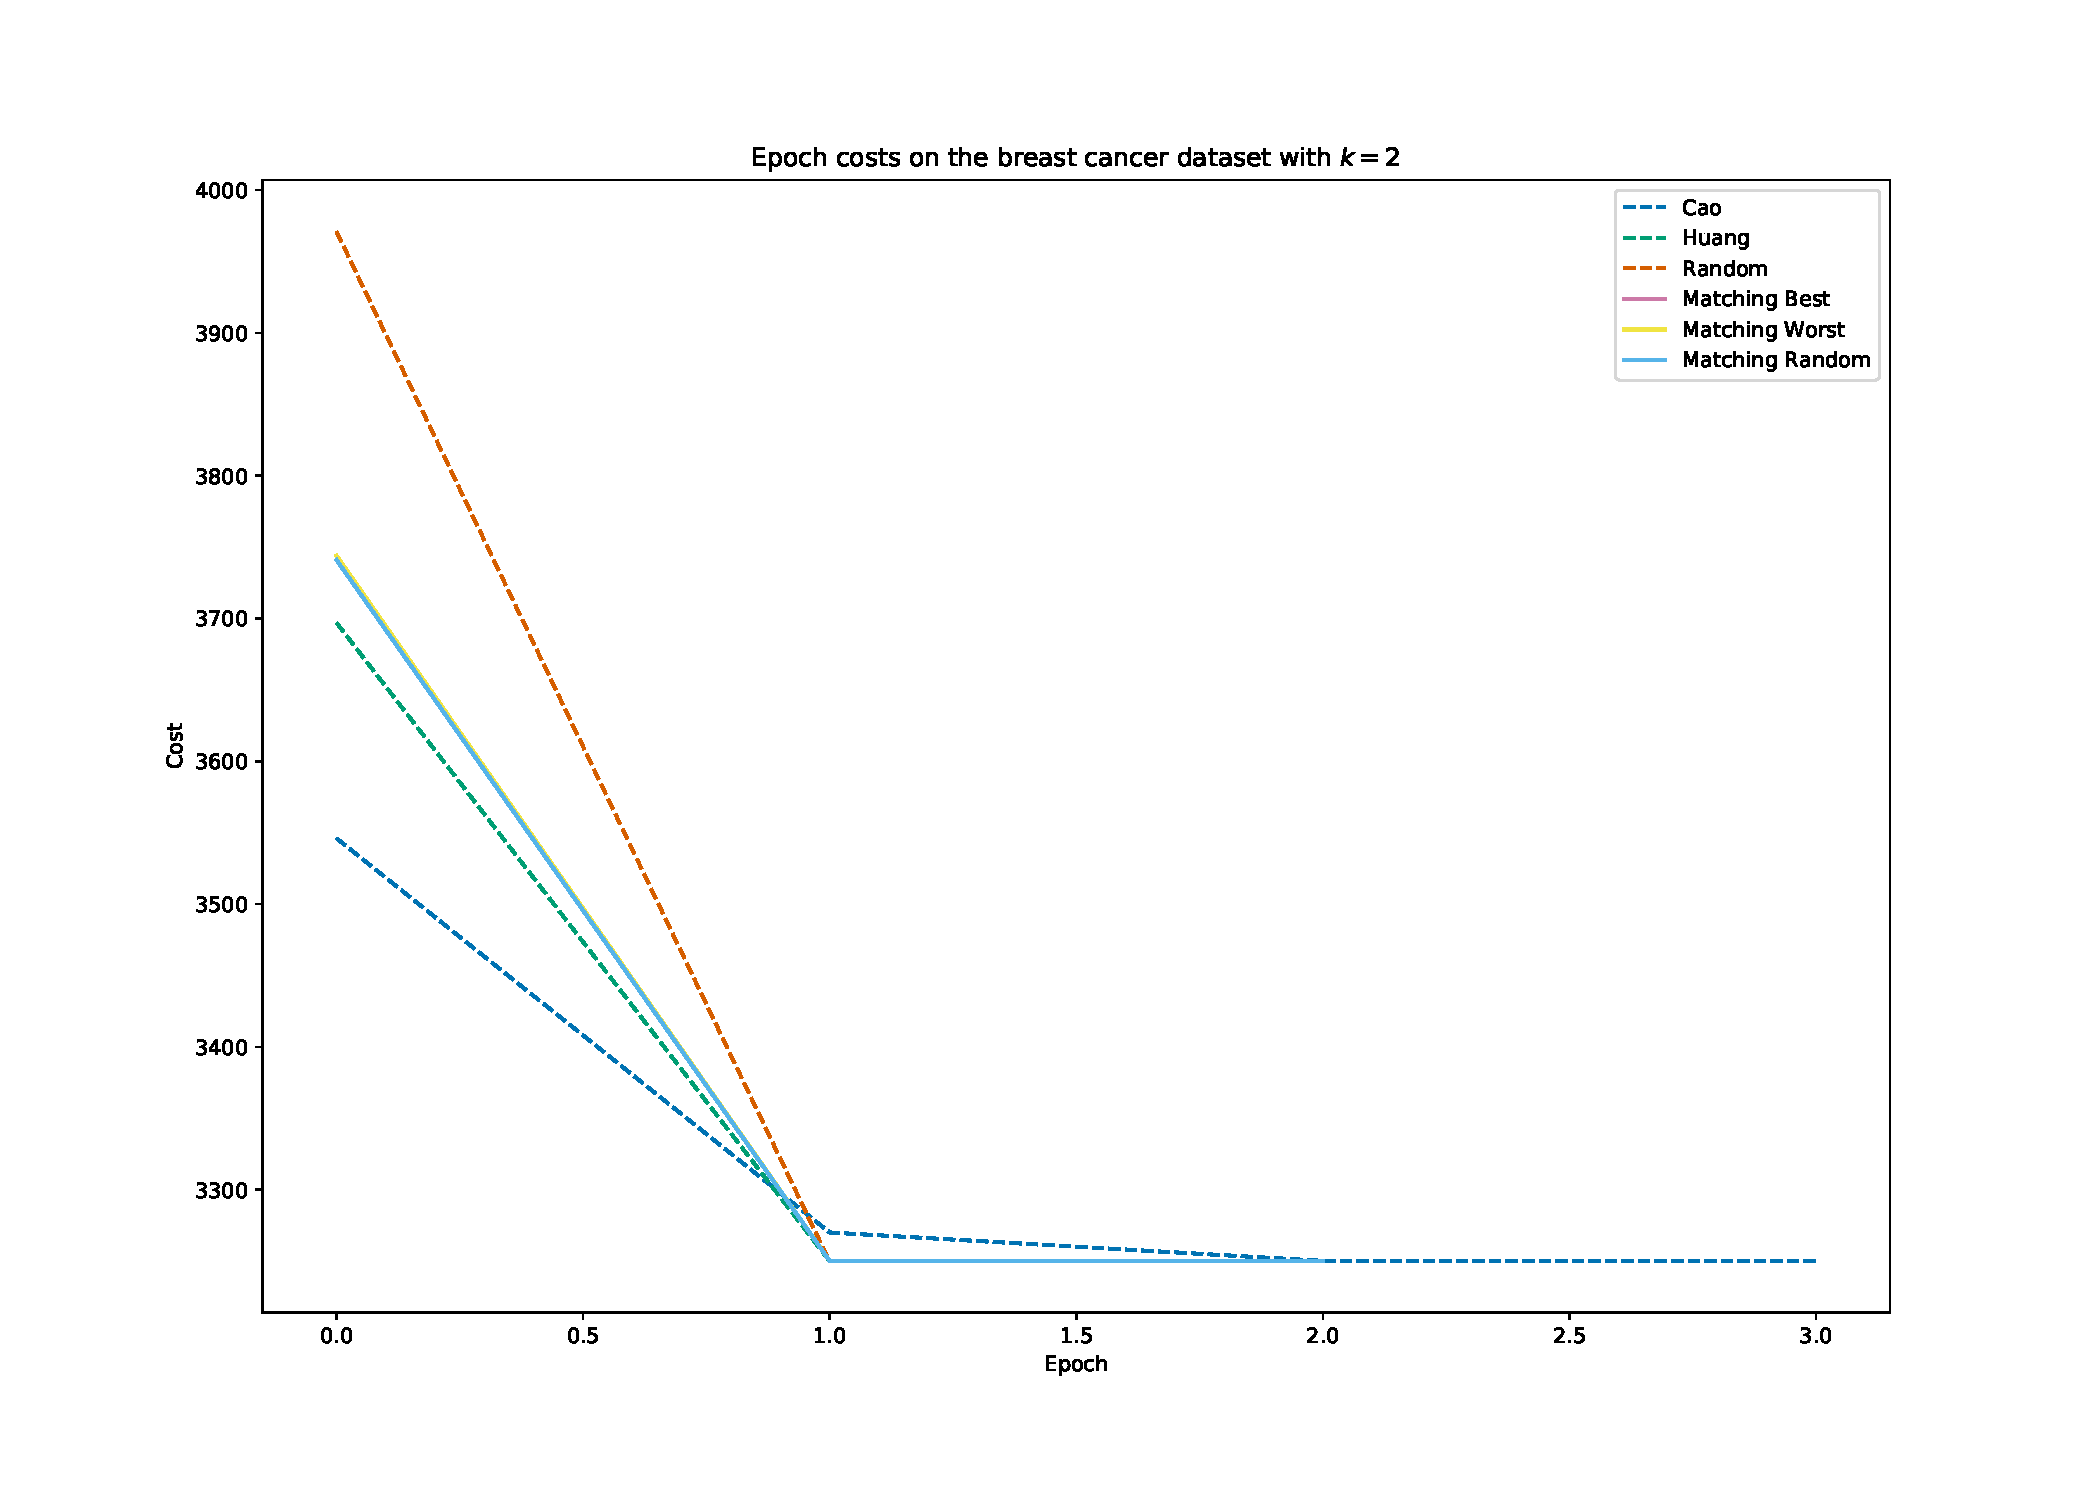
\includegraphics[width=.8\textwidth]{./img/epoch_plot_breast_cancer.pdf}
\end{figure}

\begin{figure}[h!]
    \centering
    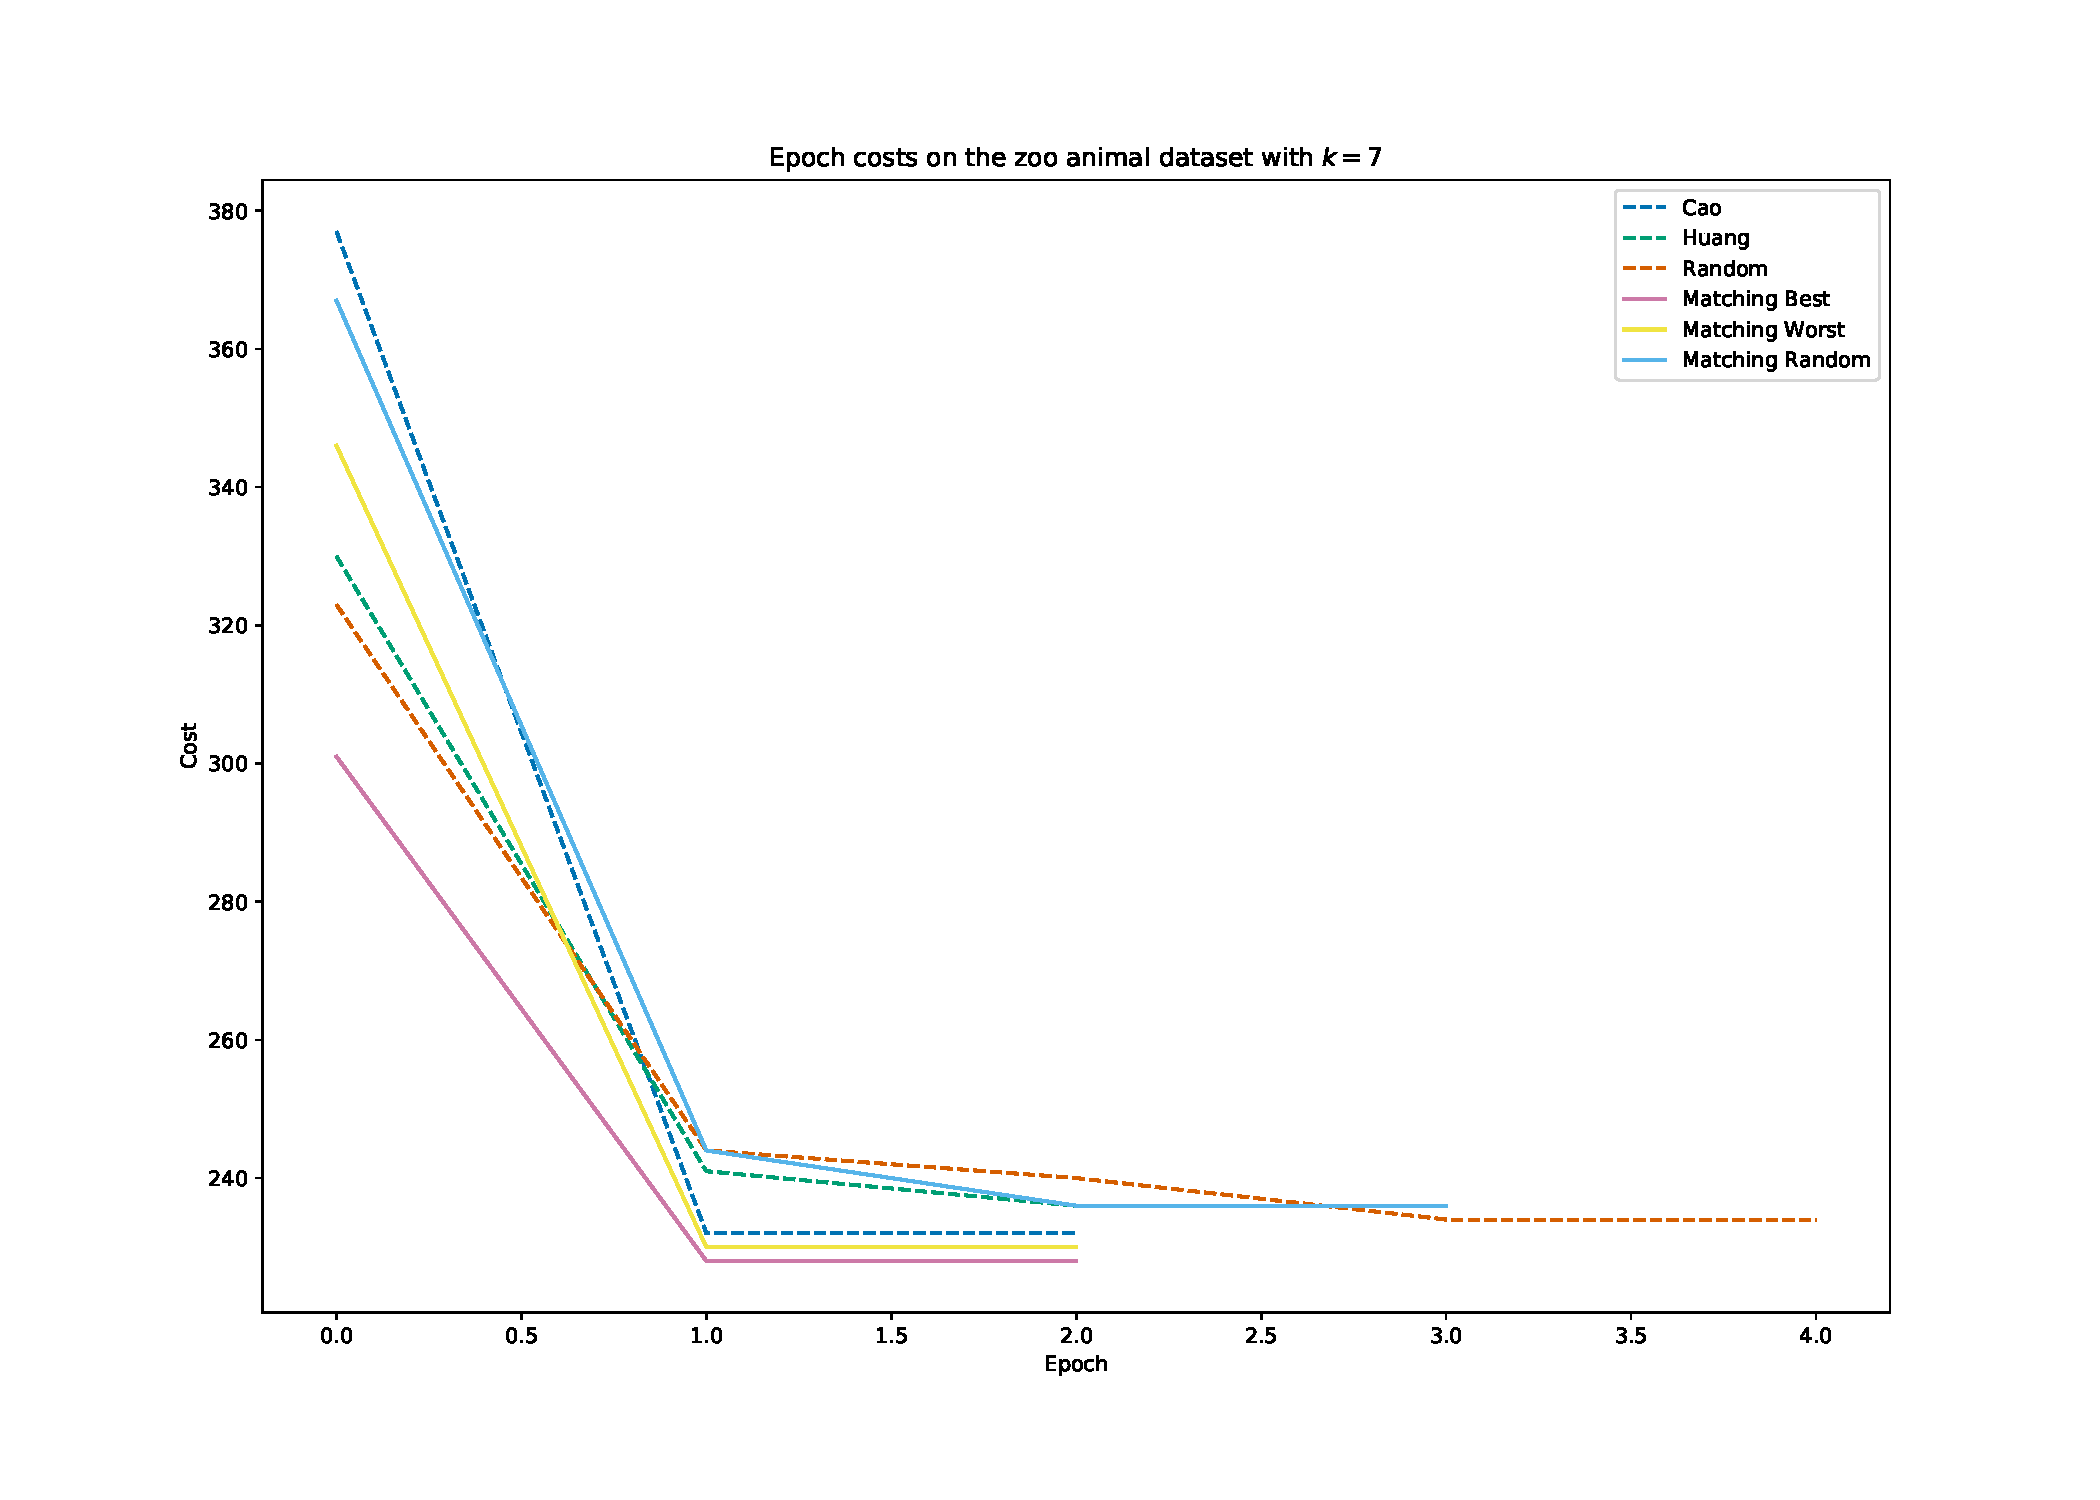
\includegraphics[width=.8\textwidth]{./img/epoch_plot_zoo_animal.pdf}
\end{figure}
